        	\begin{question}{1188}{Primitives}{1}{/}
				Que représente l'intégrale d'une fonction par rapport à $x$ entre $A$ et $B$?
            \end{question}
            \begin{reponses}
            	\item[false] La variation de la fonction entre les points $A$ et $B$
                \item[false] La longueur de la courbe de la fonction entre les points $A$ et $B$
            	\item[true] L'aire algébrique (donc possiblement négative) qui est entre la courbe de la fonction et l'axe des $x$, entre les points $A$ et $B$
                \item[false] rien de tout cela
            \end{reponses}
			%%%%%%%%%%%%%%%%%%%%%%%%%%%%%%%%%%%%%
            \begin{question}{1188}{Vecteurs}{2}{/}
                La courbe ci-dessous a pour équation $f(x)=x^2$. Combien vaut la surface délimitée par les points $A$, $B$, $C$ et $D$?
                \begin{center}
                	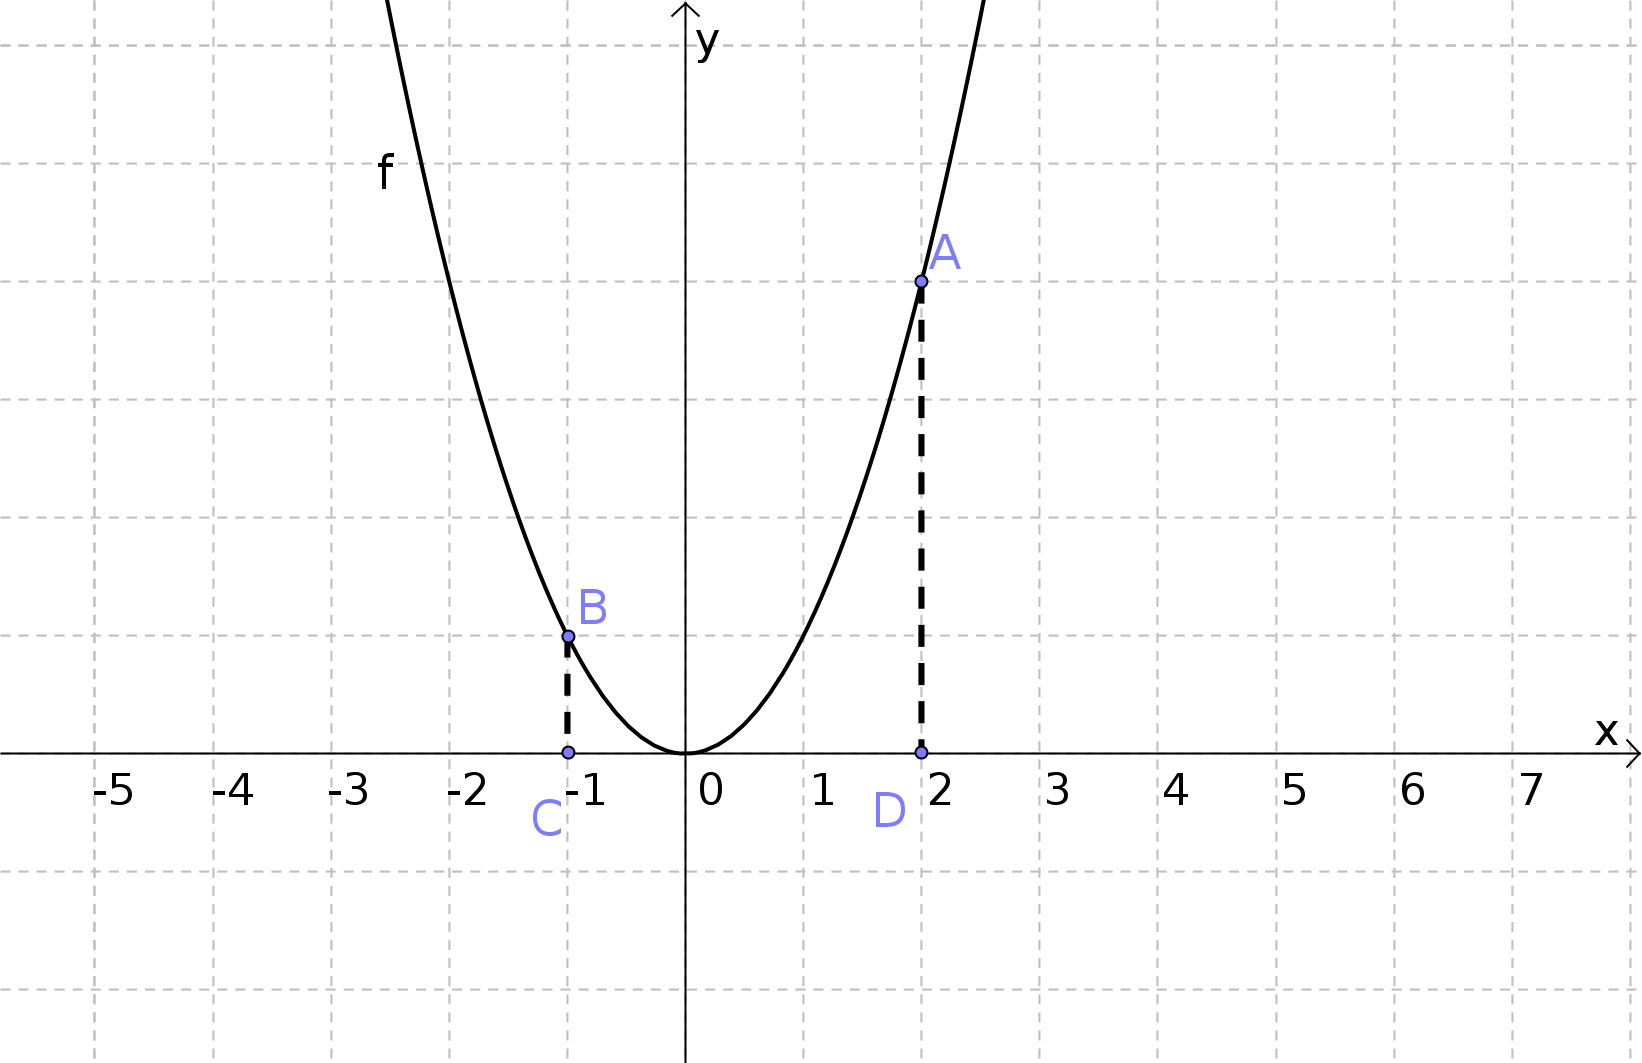
\includegraphics[width=0.5\textwidth]{Philippe/Figures_Philippe/primitives_3_2.png}
                \end{center}
            \end{question}
            \begin{reponses}
                \item[false] 3
                \item[false] $\sqrt{3}$
                \item[false] 4
                \item[true] $\sqrt{4}$ 
            \end{reponses}
            %%%%%%%%%%%%%%%%%%%%%%%%%%%%%%%%%%%%%
            \begin{question}{1188}{Primitives}{2}{/}
                Une fonction $f$ est strictement croissante sur un intervalle. Quelle affirmation est vraie sur le même intervalle?
            \end{question}
            \begin{reponses}
                \item[false] Sa primitive est négative
                \item[true] Sa primitive est positive
                \item[false] Sa primitive est nulle
                \item[false] Aucune de ces affirmations
            \end{reponses}
            %%%%%%%%%%%%%%%%%%%%%%%%%%%%%%%%%%%%%
            \begin{question}{1188}{Primitives}{2}{/}
                Supposons que nous disposions d'un graphique représentant la fonction de la puissance électrique consommée par un foyer en fonction du temps, sur une année entière. Sachant que la puissance est la dérivée de l'énergie par rapport au temps, comment fait-on pour connaître la quantité totale d'énergie consommée dans l'année?
            \end{question}
            \begin{reponses}
                \item[false] On calcule la primitive la fonction.
                \item[false] On calcule la dérivée la fonction.
                \item[true] On calcule l'intégrale la fonction.
                \item[false] On ne peut pas le faire.
            \end{reponses}
            %%%%%%%%%%%%%%%%%%%%%%%%%%%%%%%%%%%%%
